% questions.tex —— 2020 年·北京卷 · 题目内容片段（无答案）
% 由 tools/generate_projects.py 依来源总账自 2020/2020_数学真题_北京_试题.md 生成，勿手改（改源 MD 后重跑）


\begin{gknotice}
\textbf{来源说明}：本题面依据固定源 PDF 的两页 A3 题面逐题转录，原卷印刷页码为 1113、1114。第 1113 面自左至右分三栏：左栏为选择题 1—8 与第 4 题三视图；中栏为第 9、10 题与填空题 11—15（含第 15 题曲线图）；右栏为解答题 16、17（含第 16 题正方体图）。第 1114 面分三栏：左栏 18、19，中栏 20，右栏 21。全卷三处节头依次为「一、选择题」「二、填空题」「三、解答题」，题号与索引一致；所有数值、分式、根号与上下标均回原页 600—2000 dpi 核对。

\textbf{解析归属}：固定源不附答案或解析；配套答案与解析均由本库按本题面独立复算（等级 D，非官方）。

\textbf{选做说明}：第 17 题给出条件①、条件②两个条件供选用（原卷注明「如果选择条件①和条件②分别解答，按第一个解答计分」）。本库两条件全部收录并分别作答，以【条件①】【条件②】标出。

\textbf{图形说明}：第 4 题的三视图、第 15 题的污水排放曲线、第 16 题的正方体由项目内 TikZ 矢量源重绘；其余各题原页无图。

\textbf{校勘}：第 8 题原页条件为「$a_1=-9$，$a_3=-1$」；部分流传版本作 $a_5=-1$，属版本差异，本题以固定源原页的 $a_3=-1$ 为准（若按 $a_5=-1$ 则公差为 $2$、$a_n=2n-11$，结论同为「有最大项、无最小项」）。
\end{gknotice}

\gkpart{一、选择题}

\begin{question}
\gkti{1}已知集合 $A=\{-1,0,1,2\}$，$B=\{x\mid 0<x<3\}$，则 $A\cap B=$\mbox{（　　）}

（A）$\{-1,0,1\}$；（B）$\{0,1\}$；（C）$\{-1,1,2\}$；（D）$\{1,2\}$。

\end{question}
\begin{question}
\gkti{2}在复平面内，复数 $z$ 对应的点的坐标是 $(1,2)$，则 $\mathrm i\cdot z=$\mbox{（　　）}

（A）$1+2\mathrm i$；（B）$-2+\mathrm i$；（C）$1-2\mathrm i$；（D）$-2-\mathrm i$。

\end{question}
\begin{question}
\gkti{3}在 $(\sqrt x-2)^5$ 的展开式中，$x^2$ 的系数为\mbox{（　　）}

（A）$-5$；（B）$5$；（C）$-10$；（D）$10$。

\Needspace{0.4\textheight}
\end{question}
\begin{question}
\gkti{4}某三棱柱的底面为正三角形，其三视图如图所示，该三棱柱的表面积为\mbox{（　　）}

（A）$6+\sqrt3$；（B）$6+2\sqrt3$；（C）$12+\sqrt3$；（D）$12+2\sqrt3$。
\nopagebreak[4]
\begin{center}% 2020 北京卷 第 4 题：正三棱柱的三视图
% 来源 PDF：普通高考/2020/2020北京.pdf 第 1 页（A3 横排），印面 1113，第 4 题题干下方
% 原页矢量（pt，左上角为原点）：正（主）视图为 62.37 x 62.36 的正方形，中线一条竖直虚线；
%   侧（左）视图为同尺寸正方形；俯视图为底边 62.37、高 62.36 的等腰三角形（顶点在上）；
%   尺寸标注：左侧竖直双箭头「2」，主视图底边在中线处分为「1」「1」两段。
% 说明：原页三视图为示意画法（侧视图宽度与主视图相同、俯视图高等于底边），并非严格按
%   正三角形的高 sqrt3 缩放；题干另以「底面为正三角形」和尺寸 2、1、1 给出真实数据，
%   即底面正三角形边长 2、棱柱高 2。此处按原页如实重绘，不据图量取比例。
\begin{tikzpicture}[line width=0.7pt, font=\small,
  x=1.05cm, y=1.05cm, line cap=round, line join=round]

  % 正（主）视图：2 x 2 正方形 + 中线竖直虚线
  \draw (0,0) rectangle (2,2);
  \draw[dashed] (1,0) -- (1,2);

  % 侧（左）视图：2 x 2 正方形
  \draw (3,0) rectangle (5,2);

  % 俯视图：底边 2、顶点在上的等腰三角形（原页画法）
  \draw (0,-3.05) -- (2,-3.05) -- (1,-1.05) -- cycle;

  % 尺寸标注：高 2（左侧竖直双箭头）
  \draw[<->] (-0.30,0) -- (-0.30,2);
  \draw[thin] (-0.40,0) -- (0,0);
  \draw[thin] (-0.40,2) -- (0,2);
  \node[left, inner sep=3pt] at (-0.32,1) {$2$};

  % 尺寸标注：底边 1 与 1
  \draw[<->] (0,-0.24) -- (1,-0.24);
  \draw[<->] (1,-0.24) -- (2,-0.24);
  \node[below=1pt, inner sep=0pt] at (0.5,-0.24) {$1$};
  \node[below=1pt, inner sep=0pt] at (1.5,-0.24) {$1$};

  % 视图名称
  \node[below=2pt, inner sep=0pt] at (1,-0.72) {正（主）视图};
  \node[below=2pt, inner sep=0pt] at (4,-0.72) {侧（左）视图};
  \node[below=2pt, inner sep=0pt] at (1,-3.22) {俯视图};
\end{tikzpicture}
\end{center}
\nopagebreak[4]
\end{question}
\begin{question}
\gkti{5}已知半径为 $1$ 的圆经过点 $(3,4)$，则其圆心到原点的距离的最小值为\mbox{（　　）}

（A）$4$；（B）$5$；（C）$6$；（D）$7$。

\end{question}
\begin{question}
\gkti{6}已知函数 $f(x)=2^x-x-1$，则不等式 $f(x)>0$ 的解集是\mbox{（　　）}

（A）$(-1,1)$；（B）$(-\infty,-1)\cup(1,+\infty)$；（C）$(0,1)$；（D）$(-\infty,0)\cup(1,+\infty)$。

\end{question}
\begin{question}
\gkti{7}设抛物线的顶点为 $O$，焦点为 $F$，准线为 $l$。$P$ 是抛物线上异于 $O$ 的一点，过 $P$ 作 $PQ\perp l$ 于 $Q$，则线段 $FQ$ 的垂直平分线\mbox{（　　）}

（A）经过点 $O$；（B）经过点 $P$；（C）平行于直线 $OP$；（D）垂直于直线 $OP$。

\end{question}
\begin{question}
\gkti{8}在等差数列 $\{a_n\}$ 中，$a_1=-9$，$a_3=-1$。记 $T_n=a_1a_2\cdots a_n$（$n=1,2,\cdots$），则数列 $\{T_n\}$\mbox{（　　）}

（A）有最大项，有最小项；（B）有最大项，无最小项；

（C）无最大项，有最小项；（D）无最大项，无最小项。

\end{question}
\begin{question}
\gkti{9}已知 $\alpha$，$\beta\in\mathbf R$，则「存在 $k\in\mathbf Z$ 使得 $\alpha=k\pi+(-1)^k\beta$」是「$\sin\alpha=\sin\beta$」的\mbox{（　　）}

（A）充分而不必要条件；（B）必要而不充分条件；（C）充分必要条件；（D）既不充分也不必要条件。

\end{question}
\begin{question}
\gkti{10}2020 年 3 月 14 日是全球首个国际圆周率日（$\pi$ Day）。历史上，求圆周率 $\pi$ 的方法有多种，与中国传统数学中的「割圆术」相似。数学家阿尔·卡西的方法是：当正整数 $n$ 充分大时，计算单位圆的内接正 $6n$ 边形的周长和外切正 $6n$ 边形（各边均与圆相切的正 $6n$ 边形）的周长，将它们的算术平均数作为 $2\pi$ 的近似值。按照阿尔·卡西的方法，$\pi$ 的近似值的表达式是\mbox{（　　）}

（A）$3n\left(\sin\dfrac{30^\circ}{n}+\tan\dfrac{30^\circ}{n}\right)$；（B）$6n\left(\sin\dfrac{30^\circ}{n}+\tan\dfrac{30^\circ}{n}\right)$；

（C）$3n\left(\sin\dfrac{60^\circ}{n}+\tan\dfrac{60^\circ}{n}\right)$；（D）$6n\left(\sin\dfrac{60^\circ}{n}+\tan\dfrac{60^\circ}{n}\right)$。

\end{question}
\gkpart{二、填空题}

\begin{question}
\gkti{11}函数 $f(x)=\dfrac1{x+1}+\ln x$ 的定义域是\gkblank{}。

\end{question}
\begin{question}
\gkti{12}已知双曲线 $C:\dfrac{x^2}6-\dfrac{y^2}3=1$，则 $C$ 的右焦点的坐标为\gkblank{}；$C$ 的焦点到其渐近线的距离是\gkblank{}。

\end{question}
\begin{question}
\gkti{13}已知正方形 $ABCD$ 的边长为 $2$，点 $P$ 满足 $\overrightarrow{AP}=\dfrac12\left(\overrightarrow{AB}+\overrightarrow{AC}\right)$，则 $|\overrightarrow{PD}|=$\gkblank{}；$\overrightarrow{PB}\cdot\overrightarrow{PD}=$\gkblank{}。

\end{question}
\begin{question}
\gkti{14}若函数 $f(x)=\sin(x+\varphi)+\cos x$ 的最大值为 $2$，则常数 $\varphi$ 的一个取值为\gkblank{}。

\Needspace{0.4\textheight}
\end{question}
\begin{question}
\gkti{15}为满足人民对美好生活的向往，环保部门要求相关企业加强污水治理，排放未达标的企业要限期整改。设企业的污水排放量 $W$ 与时间 $t$ 的关系为 $W=f(t)$，用 $-\dfrac{f(b)-f(a)}{b-a}$ 的大小评价在 $[a,b]$ 这段时间内企业污水治理能力的强弱。已知整改期内，甲、乙两企业的污水排放量与时间的关系如图所示。
\nopagebreak[4]
\begin{center}% 2020 北京卷 第 15 题：甲、乙两企业污水排放量 W 与时间 t 的关系曲线
% 来源 PDF：普通高考/2020/2020北京.pdf 第 1 页（A3 横排），印面 1113，第 15 题题干下方
% 重绘依据：原页该图为矢量路径，已由 pdftocairo -svg 解出四条折线（两企业各被 t2 处的
%   交点切成左右两段），按坐标轴端点（O、t 轴右端、W 轴上端）线性换算为本图坐标，
%   采样后以 plot 还原，形状与原页一致。
% 原页要素：横轴 t、纵轴 W；水平虚线「污水达标排放量」；t 轴上 t1、t2、t3 三条竖直虚线
%   （t1 在甲曲线开始明显下降之后、t2 在两曲线交点、t3 在两曲线都降到达标线以下之后）；
%   曲线起点处标「甲企业」（上）、「乙企业」（下），交点右下方标「乙企业」（上）、
%   「甲企业」（下）。
\begin{tikzpicture}[line width=0.7pt, font=\small,
  x=0.50cm, y=0.50cm, line cap=round, line join=round]

  % 坐标轴（W 轴比原页留高一点，供曲线标注）
  \draw[->] (0,0) -- (15.9,0) node[below, inner sep=5pt] {$t$};
  \draw[->] (0,0) -- (0,13.4) node[right, inner sep=3pt] {$W$};
  \node[below left, inner sep=2pt] at (0,0) {$O$};

  % 污水达标排放量（水平虚线；标注按原页置于纵轴左侧）
  \draw[dashed] (0,2.92) -- (15.1,2.92);
  \node[left, inner sep=2pt] at (-0.15,2.92) {污水达标排放量};

  % 甲企业曲线（左段：起点最高，先略升后下降；右段：过交点后降得最快）
  \draw plot[smooth] coordinates {
    (0.00,8.76) (0.82,8.86) (1.63,8.87) (2.45,8.79) (3.26,8.62)
    (4.07,8.37) (4.85,8.02) (5.62,7.60) (6.37,7.08) (7.10,6.49)
    (7.79,5.82) (8.45,5.08) (9.07,4.26)
  };
  \draw plot[smooth] coordinates {
    (9.07,4.26) (9.45,3.85) (9.83,3.47) (10.23,3.12) (10.64,2.80)
    (11.06,2.51) (11.49,2.26) (11.92,2.04) (12.37,1.85) (12.81,1.70)
    (13.27,1.58) (13.72,1.50) (14.18,1.46)
  };

  % 乙企业曲线（左段：起点较低，单调缓降；右段：过交点后仍在甲之上）
  \draw plot[smooth] coordinates {
    (0.00,6.60) (0.77,6.59) (1.54,6.55) (2.31,6.47) (3.08,6.36)
    (3.84,6.22) (4.60,6.04) (5.36,5.83) (6.11,5.58) (6.86,5.30)
    (7.61,4.99) (8.34,4.64) (9.07,4.26)
  };
  \draw plot[smooth] coordinates {
    (9.07,4.26) (9.47,3.98) (9.88,3.71) (10.29,3.47) (10.71,3.24)
    (11.13,3.05) (11.56,2.87) (11.99,2.72) (12.43,2.60) (12.86,2.50)
    (13.30,2.42) (13.74,2.37) (14.18,2.34)
  };

  % t1、t2、t3 三条竖直虚线（高度分别止于对应曲线）
  \draw[dashed] (3.89,0) -- (3.89,8.58);
  \draw[dashed] (9.07,0) -- (9.07,4.26);
  \draw[dashed] (13.80,0) -- (13.80,2.39);
  \node[below, inner sep=4pt] at (3.89,0) {$t_1$};
  \node[below, inner sep=4pt] at (9.07,0) {$t_2$};
  \node[below, inner sep=4pt] at (13.80,0) {$t_3$};

  % 曲线标注（按原页位置：起点标注在曲线上方，交点后的标注在右侧）
  \node[right, inner sep=2pt] at (0.45,10.18) {甲企业};
  \node[right, inner sep=2pt] at (0.45,7.85) {乙企业};
  \node[right, inner sep=2pt] at (10.95,4.62) {乙企业};
  \node[right, inner sep=2pt] at (10.95,1.52) {甲企业};
\end{tikzpicture}
\end{center}
\nopagebreak[4]
给出下列四个结论：

① 在 $[t_1,t_2]$ 这段时间内，甲企业的污水治理能力比乙企业强；

② 在 $t_2$ 时刻，甲企业的污水治理能力比乙企业强；

③ 在 $t_3$ 时刻，甲、乙两企业的污水排放都已达标；

④ 甲企业在 $[0,t_1]$、$[t_1,t_2]$、$[t_2,t_3]$ 这三段时间中，在 $[0,t_1]$ 的污水治理能力最强。

其中所有正确结论的序号是\gkblank{}。

\end{question}
\gkpart{三、解答题}

\Needspace{0.4\textheight}
\begin{question}
\gkti{16}如图，在正方体 $ABCD-A_1B_1C_1D_1$ 中，$E$ 为 $BB_1$ 的中点。

（1） 求证：$BC_1\parallel$ 平面 $AD_1E$；

（2） 求直线 $AA_1$ 与平面 $AD_1E$ 所成角的正弦值。
\nopagebreak[4]
\begin{center}% 2020 北京卷 第 16 题：正方体 ABCD-A1B1C1D1，E 为 BB1 的中点
% 来源 PDF：普通高考/2020/2020北京.pdf 第 1 页（A3 横排），印面 1113，第 16 题右侧
% 重绘依据：原页该图为矢量路径，pdftocairo -svg 解出全部端点后按棱长归一化逐个还原。
%   原页画法：前侧面为正方形 D1C1CD（D 在左下、C 在右下、C1 在右上、D1 在左上），
%   深度方向朝右上（斜二测，长度约为棱长的一半）；后侧面 A1B1BA 与前侧面平行，
%   A 是被遮挡的顶点，故 AA1、AB、AD、AD1、AE 画虚线，D1E 亦为虚线；
%   E 位于 BB1 的中点。
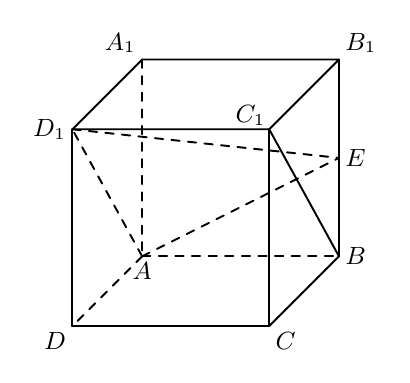
\begin{tikzpicture}[line width=0.7pt, font=\small,
  x=1.25cm, y=1.25cm, line cap=round, line join=round]

  % 顶点坐标（棱长 2，深度偏移 (0.709, 0.709)）
  \coordinate (D)  at (0.000, 0.000);
  \coordinate (C)  at (2.000, 0.000);
  \coordinate (C1) at (2.000, 2.000);
  \coordinate (D1) at (0.000, 2.000);
  \coordinate (A)  at (0.709, 0.709);
  \coordinate (B)  at (2.709, 0.709);
  \coordinate (B1) at (2.709, 2.709);
  \coordinate (A1) at (0.709, 2.709);
  \coordinate (E)  at (2.709, 1.709);

  % 上底面四边（实线）
  \draw (A1) -- (B1) -- (C1) -- (D1) -- cycle;

  % 可见棱（实线）
  \draw (D1) -- (D);
  \draw (C1) -- (C);
  \draw (D) -- (C);
  \draw (B1) -- (B);
  \draw (B) -- (C);
  \draw (B) -- (C1);

  % 被遮挡的棱与体内连线（虚线）
  \draw[dashed] (A1) -- (A);
  \draw[dashed] (A) -- (B);
  \draw[dashed] (A) -- (D);
  \draw[dashed] (A) -- (D1);
  \draw[dashed] (A) -- (E);
  \draw[dashed] (D1) -- (E);

  % 顶点标注
  \node[above left, inner sep=2pt]  at (A1) {$A_1$};
  \node[above right, inner sep=2pt] at (B1) {$B_1$};
  \node[above left, inner sep=1pt]  at (C1) {$C_1$};
  \node[left, inner sep=2pt]        at (D1) {$D_1$};
  \node[below, inner sep=2pt]       at (A)  {$A$};
  \node[right, inner sep=2pt]       at (B)  {$B$};
  \node[below right, inner sep=2pt] at (C)  {$C$};
  \node[below left, inner sep=2pt]  at (D)  {$D$};
  \node[right, inner sep=2pt]       at (E)  {$E$};
\end{tikzpicture}
\end{center}
\nopagebreak[4]
\end{question}
\begin{question}
\gkti{17}在 $\triangle ABC$ 中，$a+b=11$，再从条件①、条件②这两个条件中选择一个作为已知，求：

（1） $a$ 的值；

（2） $\sin C$ 和 $\triangle ABC$ 的面积。

条件①：$c=7$，$\cos A=-\dfrac17$；

条件②：$\cos A=\dfrac18$，$\cos B=\dfrac9{16}$。

注：如果选择条件①和条件②分别解答，按第一个解答计分。

\end{question}
\begin{question}
\gkti{18}某校为举办甲、乙两项不同活动，分别设计了相应的活动方案：方案一、方案二。为了解该校学生对活动方案是否支持，对学生进行简单随机抽样，获得数据如下表：

\begin{center}
\begin{tabular}{ccccc}
\toprule
 & 男生 &  & 女生 &  \\
\midrule
 & 支持 & 不支持 & 支持 & 不支持 \\
方案一 & $200$ 人 & $400$ 人 & $300$ 人 & $100$ 人 \\
方案二 & $350$ 人 & $250$ 人 & $150$ 人 & $250$ 人 \\
\bottomrule
\end{tabular}
\end{center}

假设所有学生对活动方案是否支持相互独立。

（1） 分别估计该校男生支持方案一的概率、该校女生支持方案一的概率；

（2） 从该校全体男生中随机抽取 $2$ 人，全体女生中随机抽取 $1$ 人，估计这 $3$ 人中恰有 $2$ 人支持方案一的概率；

（3） 将该校学生支持方案的概率估计值记为 $p_0$，假设该校年级有 $500$ 名男生和 $300$ 名女生，除一年级外其他年级学生支持方案二的概率估计值记为 $p_1$，试比较 $p_0$ 与 $p_1$ 的大小。（结论不要求证明）

\end{question}
\begin{question}
\gkti{19}已知函数 $f(x)=12-x^2$。

（1） 求曲线 $y=f(x)$ 的斜率等于 $-2$ 的切线方程；

（2） 设曲线 $y=f(x)$ 在点 $(t,f(t))$ 处的切线与坐标轴围成的三角形的面积为 $S(t)$，求 $S(t)$ 的最小值。

\end{question}
\begin{question}
\gkti{20}已知椭圆 $C:\dfrac{x^2}{a^2}+\dfrac{y^2}{b^2}=1$ 过点 $A(-2,-1)$，且 $a=2b$。

（1） 求椭圆 $C$ 的方程；

（2） 过点 $B(-4,0)$ 的直线 $l$ 交椭圆 $C$ 于点 $M$，$N$，直线 $MA$，$NA$ 分别交直线 $x=-4$ 于点 $P$，$Q$。求 $\dfrac{|PB|}{|BQ|}$ 的值。

\end{question}
\begin{question}
\gkti{21}已知 $\{a_n\}$ 是无穷数列。给出两个性质：

① 对于 $\{a_n\}$ 中任意两项 $a_i$，$a_j$（$i>j$），在 $\{a_n\}$ 中都存在一项 $a_m$，使 $\dfrac{a_i^2}{a_j}=a_m$；

② 对于 $\{a_n\}$ 中任意项 $a_n$（$n\geqslant3$），在 $\{a_n\}$ 中都存在两项 $a_k$，$a_l$（$k>l$），使得 $a_n=\dfrac{a_k^2}{a_l}$。

（1） 若 $a_n=n$（$n=1,2,\cdots$），判断数列 $\{a_n\}$ 是否满足性质①，说明理由；

（2） 若 $a_n=2^{n-1}$（$n=1,2,\cdots$），判断数列 $\{a_n\}$ 是否同时满足性质①和性质②，说明理由；

（3） 若 $\{a_n\}$ 是递增数列，且同时满足性质①和性质②，证明：$\{a_n\}$ 为等比数列。

\end{question}